% !TEX root = 99_main.tex

To study the electricity generation and building energy consumption, a 3D geometry of the room and solar facade is built using the Rhinoceros software \cite{Rhino}, and its parametric modelling plugin Grasshopper \cite{grasshopper}. The solar facade consists of 400mm CIGS square panels that can rotate in two degrees of freedom. On the horizontal axis the panels can move from 0$^{\circ}$ (closed) to 90$^{\circ}$ (open) position in steps of 22.5$^{\circ}$. In the vertical axis it can move from 45$^{\circ}$ to -45$^{\circ}$ in 22.5$^{\circ}$ steps. Existing ASF systems \cite{nagy2015frontiers} have independently actuated panels and a continuous range of actuation, however for simplicity we group all panels into one cluster that moves in unison. This leaves us with 25 possible dynamic configurations of the facade system. 

The building energy simulation is conducted using EnergyPlus \cite{energyplus} through the DIVA \cite{DIVA} interface. The geometric solar facade is interpreted in EnergyPlus as an external shading system. A solar radiance simulation is run in parallel with Ladybug \cite{roudsari2014ladybug}  which uses Radiance \cite{ward1994radiance} to determine the incident insolation on the solar facade. The approach enables us to calculate solar irradiance on the modules with high spatial resolution including the effect of module mutual shading as seen in Figure \ref{fig:radiation}. The results are coupled to an electrical circuit simulation of thin-film PV modules with sub-cell level representation \cite{hofer2015PVSEC}.

A simulation of each possible dynamic configuration of the facade is run for each hourly timestep of the year using using a weather file for Geneva, Switzerland \cite{genevaweatherfile}. The results are then post processed in Python \cite{python} to extract the configurations that minimise building energy consumption and maximise PV electricity production. A corresponding workflow can be seen in Figure \ref{fig:workflow}. 

%Johanes Comment for cyan text- This describes how it has been previously done. Please check the Ladybug/Radiance method used now and quickly describe it (calculation cumulative sky matrix for diffuse and beam radiation, etc). 


%  A cumulative sky matrix consisting of diffuse and direct radiation is calculated from the Geneva weather file \cite{genevaweatherfile} . This can be then used 
% \textcolor{cyan}{Reflected and diffuse light are taken into account using the global radiation data, visible sky fraction for each panel, and the reflection of surrounding elements - See Comments}.

% \begin{tikzpicture}[node distance = 3cm, auto]
% 	\node [decision] (rhino) {Rhino / Grasshopper};
% 	\node [block, left of=rhino] (geo) {Solar Facade Geometry};
% 	\node [block, below of=geo] (building) {Building Geometry};
% \end{tikzpicture}

% \begin{tikzpicture}[node distance = 2cm, auto]
%     % Place nodes
%     \node [block] (init) {initialize model};
%     \node [cloud, left of=init] (expert) {expert};
%     \node [cloud, right of=init] (system) {system};
%     \node [block, below of=init] (identify) {identify candidate models};
%     \node [block, below of=identify] (evaluate) {evaluate candidate models};
%     \node [block, left of=evaluate, node distance=3cm] (update) {update model};
%     \node [decision, below of=evaluate] (decide) {is best candidate better?};
%     \node [block, below of=decide, node distance=3cm] (stop) {stop};
%     % Draw edges
%     \path [line] (init) -- (identify);
%     \path [line] (identify) -- (evaluate);
%     \path [line] (evaluate) -- (decide);
%     \path [line] (decide) -| node [near start] {yes} (update);
%     \path [line] (update) |- (identify);
%     \path [line] (decide) -- node {no}(stop);
%     \path [line,dashed] (expert) -- (init);
%     \path [line,dashed] (system) -- (init);
%     \path [line,dashed] (system) |- (evaluate);
% \end{tikzpicture}

\begin{figure}
\begin{center}
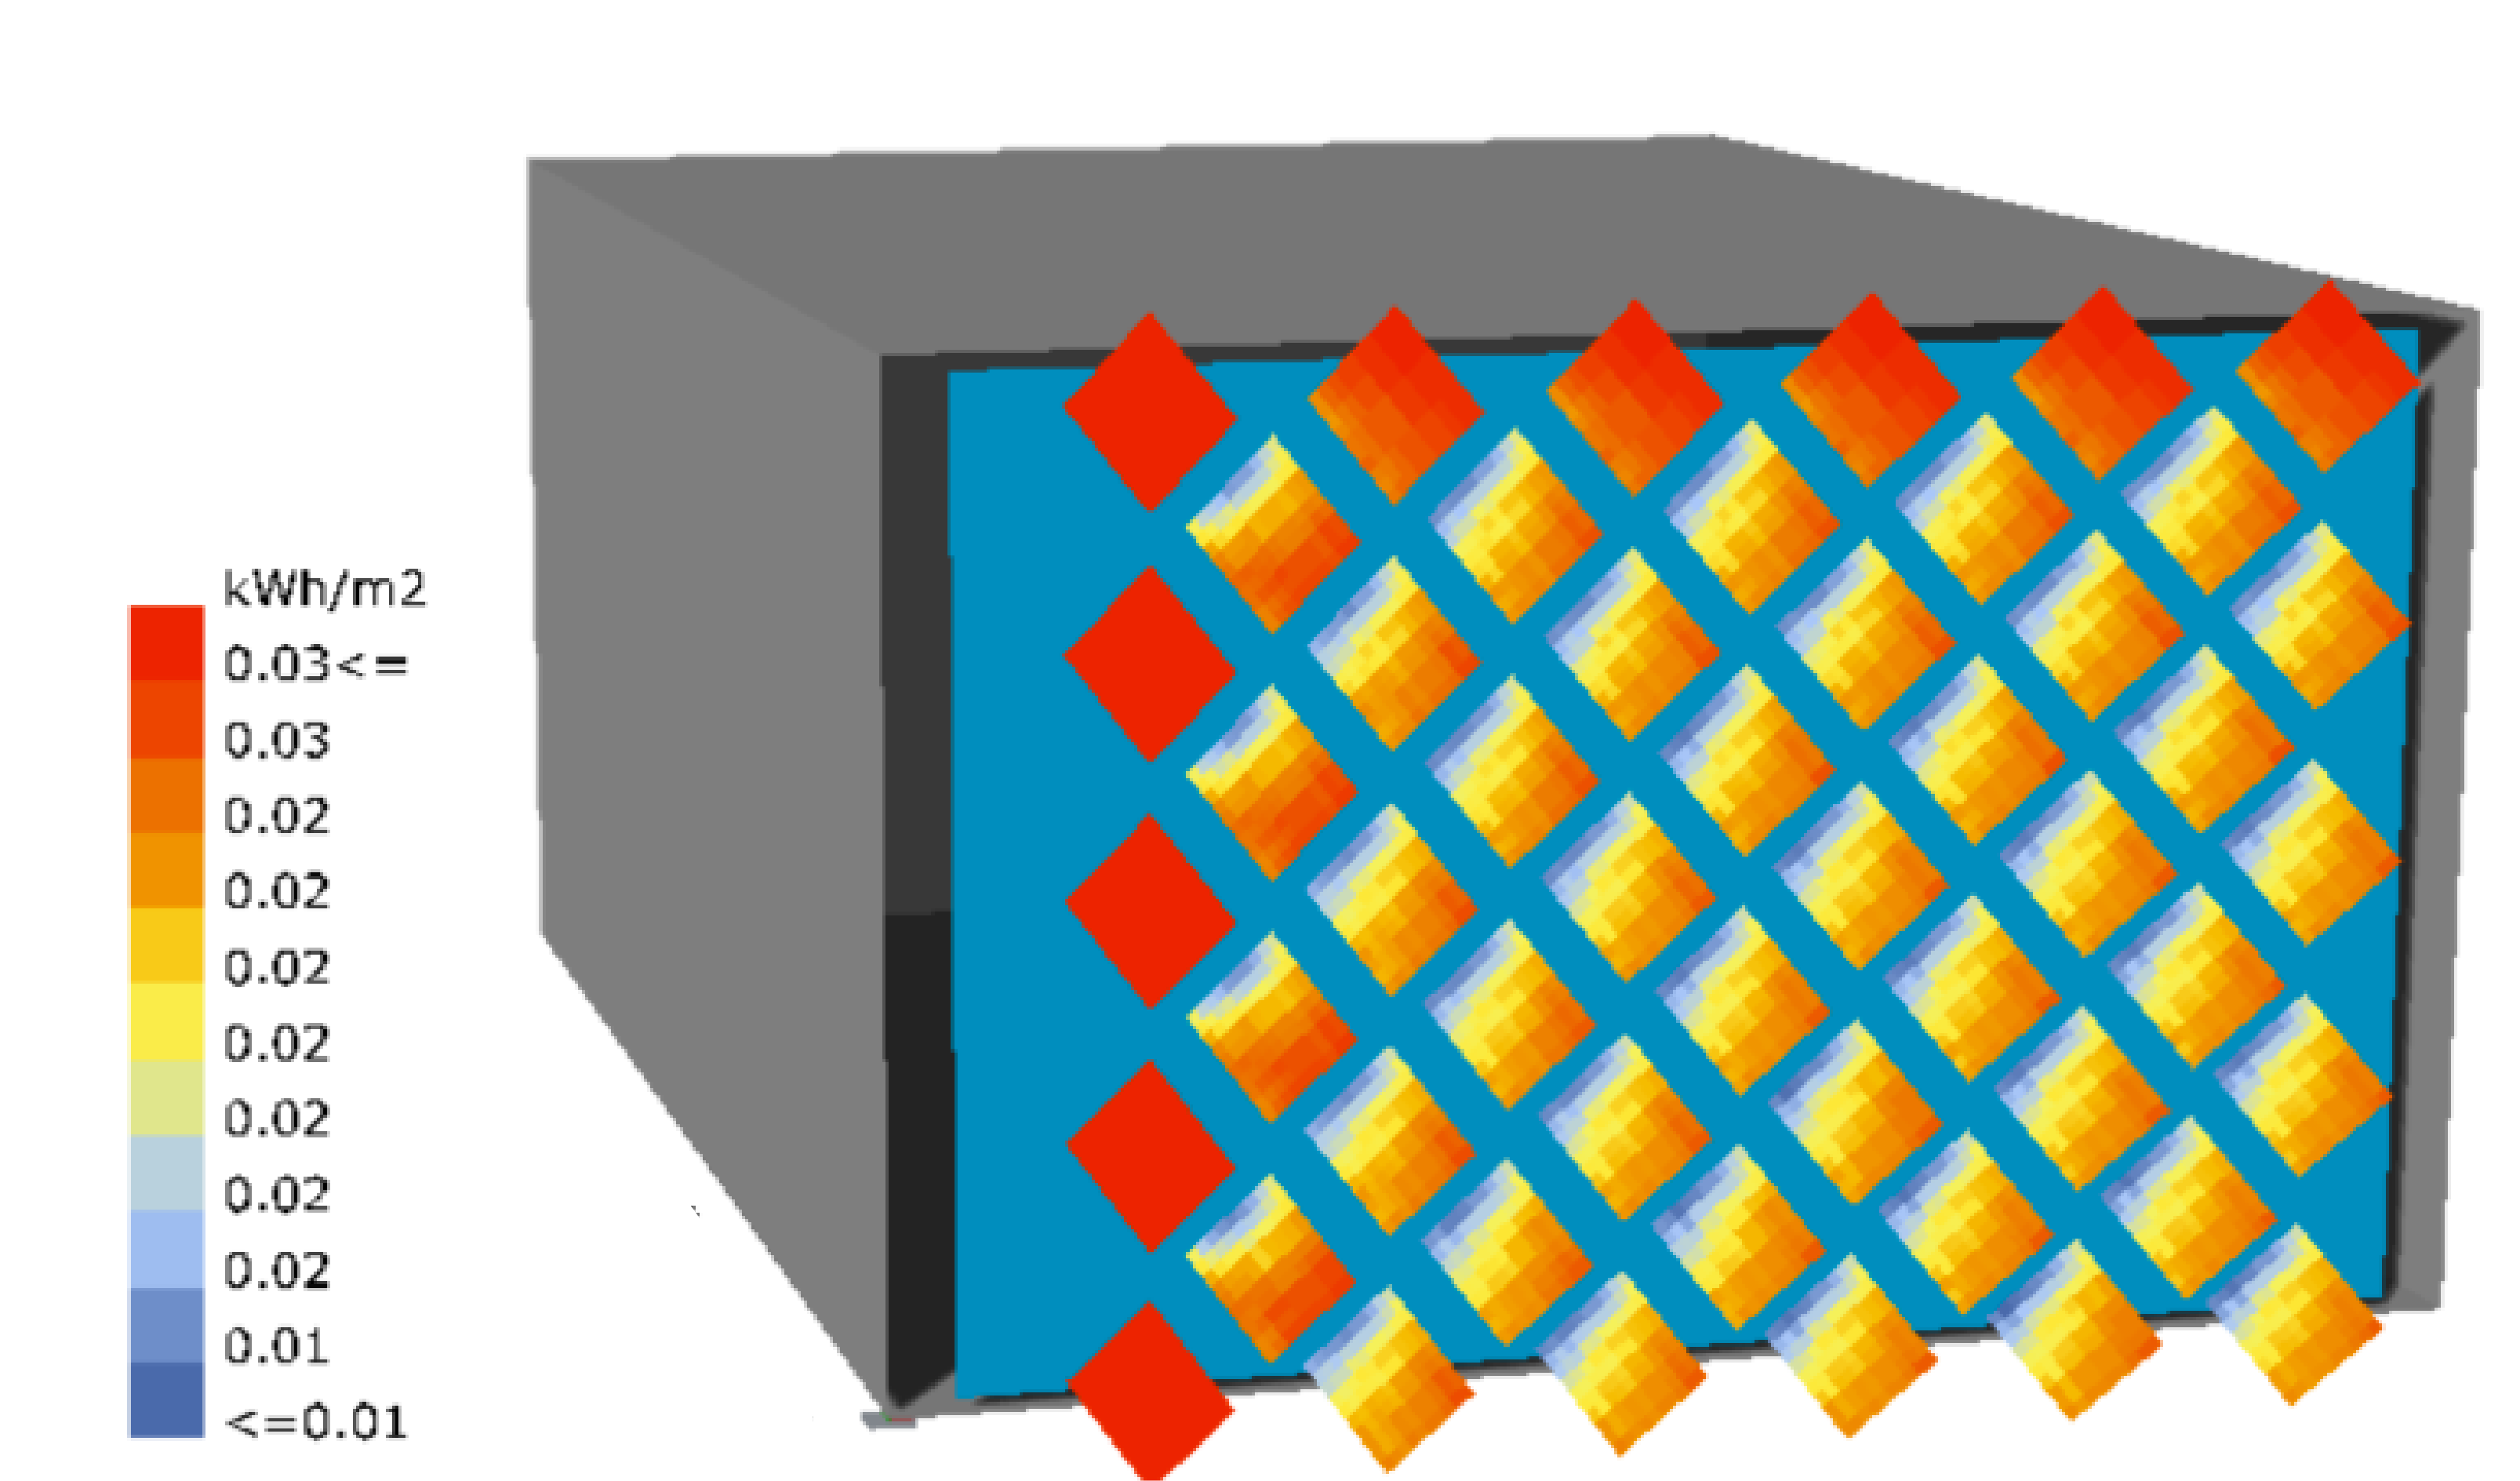
\includegraphics[width=10cm, trim= 0cm 0cm 0cm 0cm,clip]{radiationanalysis.png}
\caption{A simulation result showing module insolation from 14:00-15:00 on the 1st of January for the used weather file and a specific module orientation.}
\label{fig:radiation}
\end{center}
\end{figure}


\begin{figure}
\begin{center}
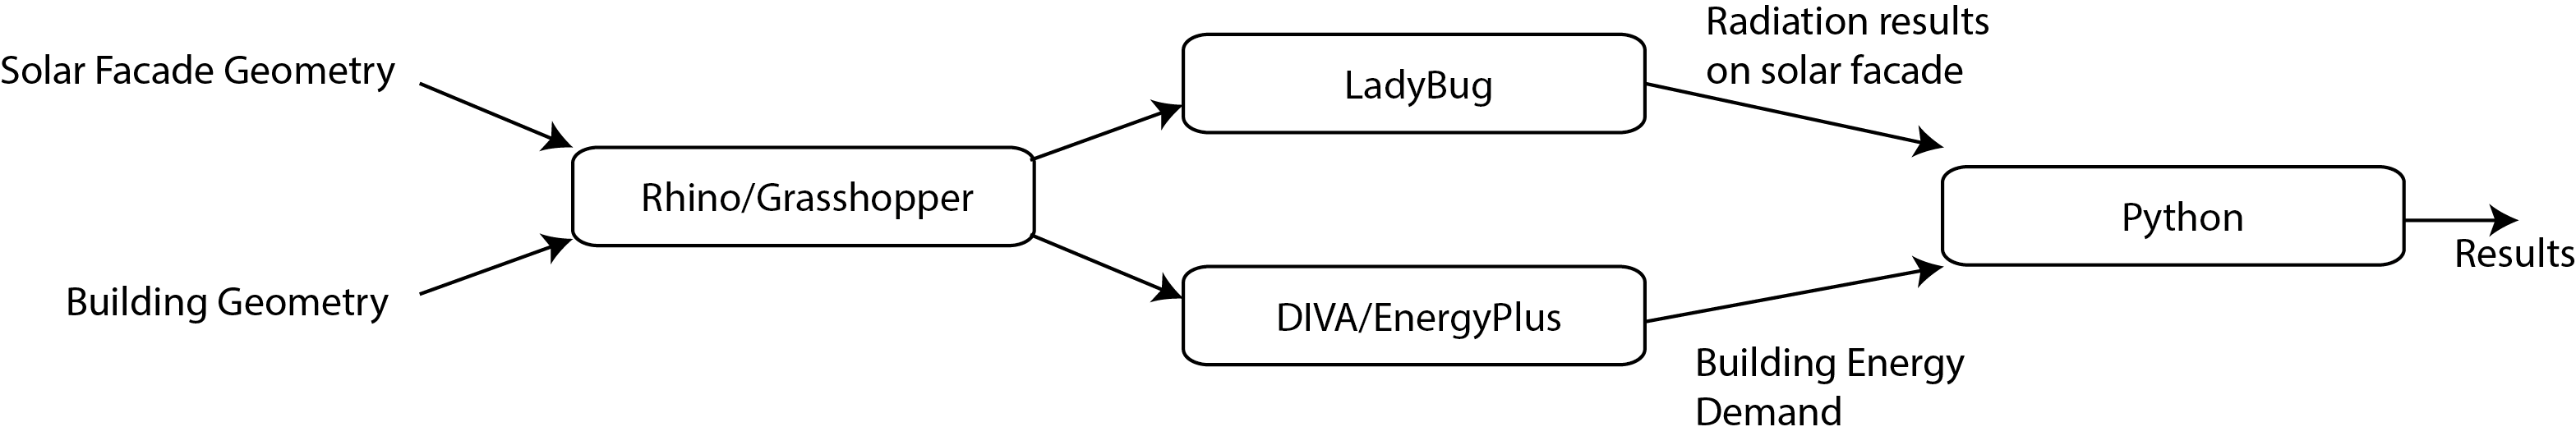
\includegraphics[width=15cm, trim= 0cm 0cm 0cm 0cm,clip]{workflow.png}
\caption{Simulation Workflow}
\label{fig:workflow}
\end{center}
\end{figure}